% !TEX TS-program = pdflatex
% !TEX encoding = UTF-8 Unicode

% This is a simple template for a LaTeX document using the "article" class.
% See "book", "report", "letter" for other types of document.

\documentclass[8pt]{article} % use larger type; default would be 10pt

\usepackage[utf8]{inputenc} % set input encoding (not needed with XeLaTeX)
\usepackage{bchart}
\usepackage{longtable}
\usepackage{pgfgantt}
\usepackage{calendar} % Use the calendar.sty style
\usepackage{calc}
\usepackage{ifthen}
\usepackage{tkz-base}
\usepackage{tikz}
\usepackage{hyperref}
\usepackage{tkz-kiviat,numprint,fullpage} 
\usepackage{pgfplotstable} 
\usepackage{pdfpages} 
\usepackage{tikz-3dplot}
\usetikzlibrary{arrows}
\RequirePackage{pgfcalendar}
\RequirePackage{tikz}
\usetikzlibrary{%
arrows, backgrounds, calc,%
patterns, shadows, trees,positioning, shapes.geometric%
}
%\usetikzlibrary{arrows,shapes,positioning,shadows,trees}

%%% Examples of Article customizations
% These packages are optional, depending whether you want the features they provide.
% See the LaTeX Companion or other references for full information.

\usepackage{textcomp}
%\usepackage{hyperref}

%%% PAGE DIMENSIONS
\usepackage{geometry} % to change the page dimensions
\geometry{a4paper} % or letterpaper (US) or a5paper or....
% \geometry{margin=2in} % for example, change the margins to 2 inches all round
% \geometry{landscape} % set up the page for landscape
%   read geometry.pdf for detailed page layout information

\usepackage{graphicx} % support the \includegraphics command and options

% \usepackage[parfill]{parskip} % Activate to begin paragraphs with an empty line rather than an indent

%%% PACKAGES
\usepackage{booktabs} % for much better looking tables
\usepackage{array} % for better arrays (eg matrices) in maths
\usepackage{paralist} % very flexible & customisable lists (eg. enumerate/itemize, etc.)
\usepackage{verbatim} % adds environment for commenting out blocks of text & for better verbatim
\usepackage{subfig} % make it possible to include more than one captioned figure/table in a single float
% These packages are all incorporated in the memoir class to one degree or another...

%%% HEADERS & FOOTERS
\usepackage{fancyhdr} % This should be set AFTER setting up the page geometry
\pagestyle{fancy} % options: empty , plain , fancy
\renewcommand{\headrulewidth}{0pt} % customise the layout...
\lhead{}\chead{}\rhead{}
\lfoot{}\cfoot{\thepage}\rfoot{}

%%% SECTION TITLE APPEARANCE
\usepackage{sectsty}
\allsectionsfont{\sffamily\mdseries\upshape} % (See the fntguide.pdf for font help)
% (This matches ConTeXt defaults)

%%% ToC (table of contents) APPEARANCE
\usepackage[nottoc,notlof,notlot]{tocbibind} % Put the bibliography in the ToC
\usepackage[titles,subfigure]{tocloft} % Alter the style of the Table of Contents
\renewcommand{\cftsecfont}{\rmfamily\mdseries\upshape}
\renewcommand{\cftsecpagefont}{\rmfamily\mdseries\upshape} % No bold!
\usepackage{listings}
\usepackage{xcolor}
\usepackage[subsection]{placeins}
%%\usepackage{flafter}

\definecolor{codegreen}{rgb}{1,0,0}
\definecolor{codegray}{rgb}{0.5,0.5,0.5}
\definecolor{codepurple}{rgb}{0.58,0,0.82}
\definecolor{backcolour}{rgb}{0.95,0.95,0.92}

\lstdefinestyle{mystyle}{
    backgroundcolor=\color{backcolour},
    commentstyle=\color{codegreen},
    keywordstyle=\color{magenta},
    numberstyle=\tiny\color{codegray},
    stringstyle=\color{codepurple},
    basicstyle=\ttfamily\footnotesize,
    breakatwhitespace=false,
    breaklines=true,
    captionpos=b,
    keepspaces=true,
    numbers=left,
    numbersep=5pt,
    showspaces=false,
    showstringspaces=false,
    showtabs=false,
    tabsize=2
}
\lstset{style=mystyle}


%%% END Article customizations

%%% The "real" document content comes below...

\title{Project management}
\author{\copyright Frederic Kerdraon, Toto}
%\date{} % Activate to display a given date or no date (if empty),
         % otherwise the current date is printed 

\begin{document}


\maketitle
\hspace*{-1cm}\includegraphics[width=.2\textwidth]{Logo.png}
\tableofcontents

\section{Introduction}

This document summurizes all the important informations necessary to facilitate things and remove a lot of stress. It's been put together thanks to \LaTeX. This is designed to help make optimal decisions for a not so short lifetime.

%{\footnote
%Ce n'est pas parceque les choses sont difficiles que nous n'osons pas, c'est parceque nous n'osons pas qu'elles sont difficiles
%}
%{\footnote
%For once you have tasted flight you will walk the earth with your eyes turned skywards, 
%for there you have been and there you will long to return.
%Leonardo da Vinci
%
%}
%\makebox[2\width]{hello}

\newcounter{a}
\newcounter{b}

%----------------------------------------------------------
\newcommand{\slice}[4]{
  \pgfmathparse{0.5*#1+0.5*#2}
  \let\midangle\pgfmathresult

   slice
  \draw[thick,fill=black!10] (0,0) -- (#1:1) arc (#1:#2:1) -- cycle;

   outer label
  \node[label=\midangle:#4] at (\midangle:1) {};

   inner label
  \pgfmathparse{min((#2-#1-10)/110*(-0.3),0)}
  \let\temp\pgfmathresult
  \pgfmathparse{max(\temp,-0.5) + 0.8}
  \let\innerpos\pgfmathresult
  \node at (\midangle:\innerpos) {#3};
}

\section{Management summary}

%Before starting a new project, you'd better find some supporters...\\
%\begin{figure}[ht!]
%\centering
%\includegraphics[width=90mm]{World3.png}
%\caption{Connections \label{overflow}}
%\end{figure}

%{\footnote
%En gros tous les dossiers que j'ai au bureau....;-)
%}


\subsection{Summary}

%\includegraphics[width=120mm]{SeismicSphere.pdf}
%\includepdf{SeismicSphere.pdf}
%\input{SeismicSphere}

%\subsubsection{A decision tree}
%\includegraphics{Multiplot.png}
%\includepdf{MultiPlot.pdf}

%\subsubsection{Multiplot}
%\includegraphics[width=120mm]{SeismicSphere.pdf}
%\includepdf{MultiPlot.pdf}

%\subsubsection{Scatter2}
%\includegraphics[width=120mm]{SeismicSphere.pdf}
%\includepdf{Scatter2.pdf}

%\subsubsection{Regressoin}
%\includegraphics[width=120mm]{SeismicSphere.pdf}
%\includepdf{Regression.pdf}

%\subsubsection{The Workflow}
%\includegraphics[width=120mm]{SeismicSphere.pdf}
%Removed because it's UGLY\\
%\includepdf{RuleBasedTree.pdf}

\subsubsection{The green side first !}
Tasks we have completed in time\\
Good news for the project\\
New resources\\
New budget\\

\subsubsection{The challenges ahead !}
Highest investment or Budget (time and monney)\\
Tasks that we couldnt complete in time\\
Resources that need to move their asses\\
Tasks that we dont want to fuck up (critical path of the highest investment)\\

\clearpage
\subsubsection{The Project timeline}
The gantt chart of the project\\
\begin{center}
%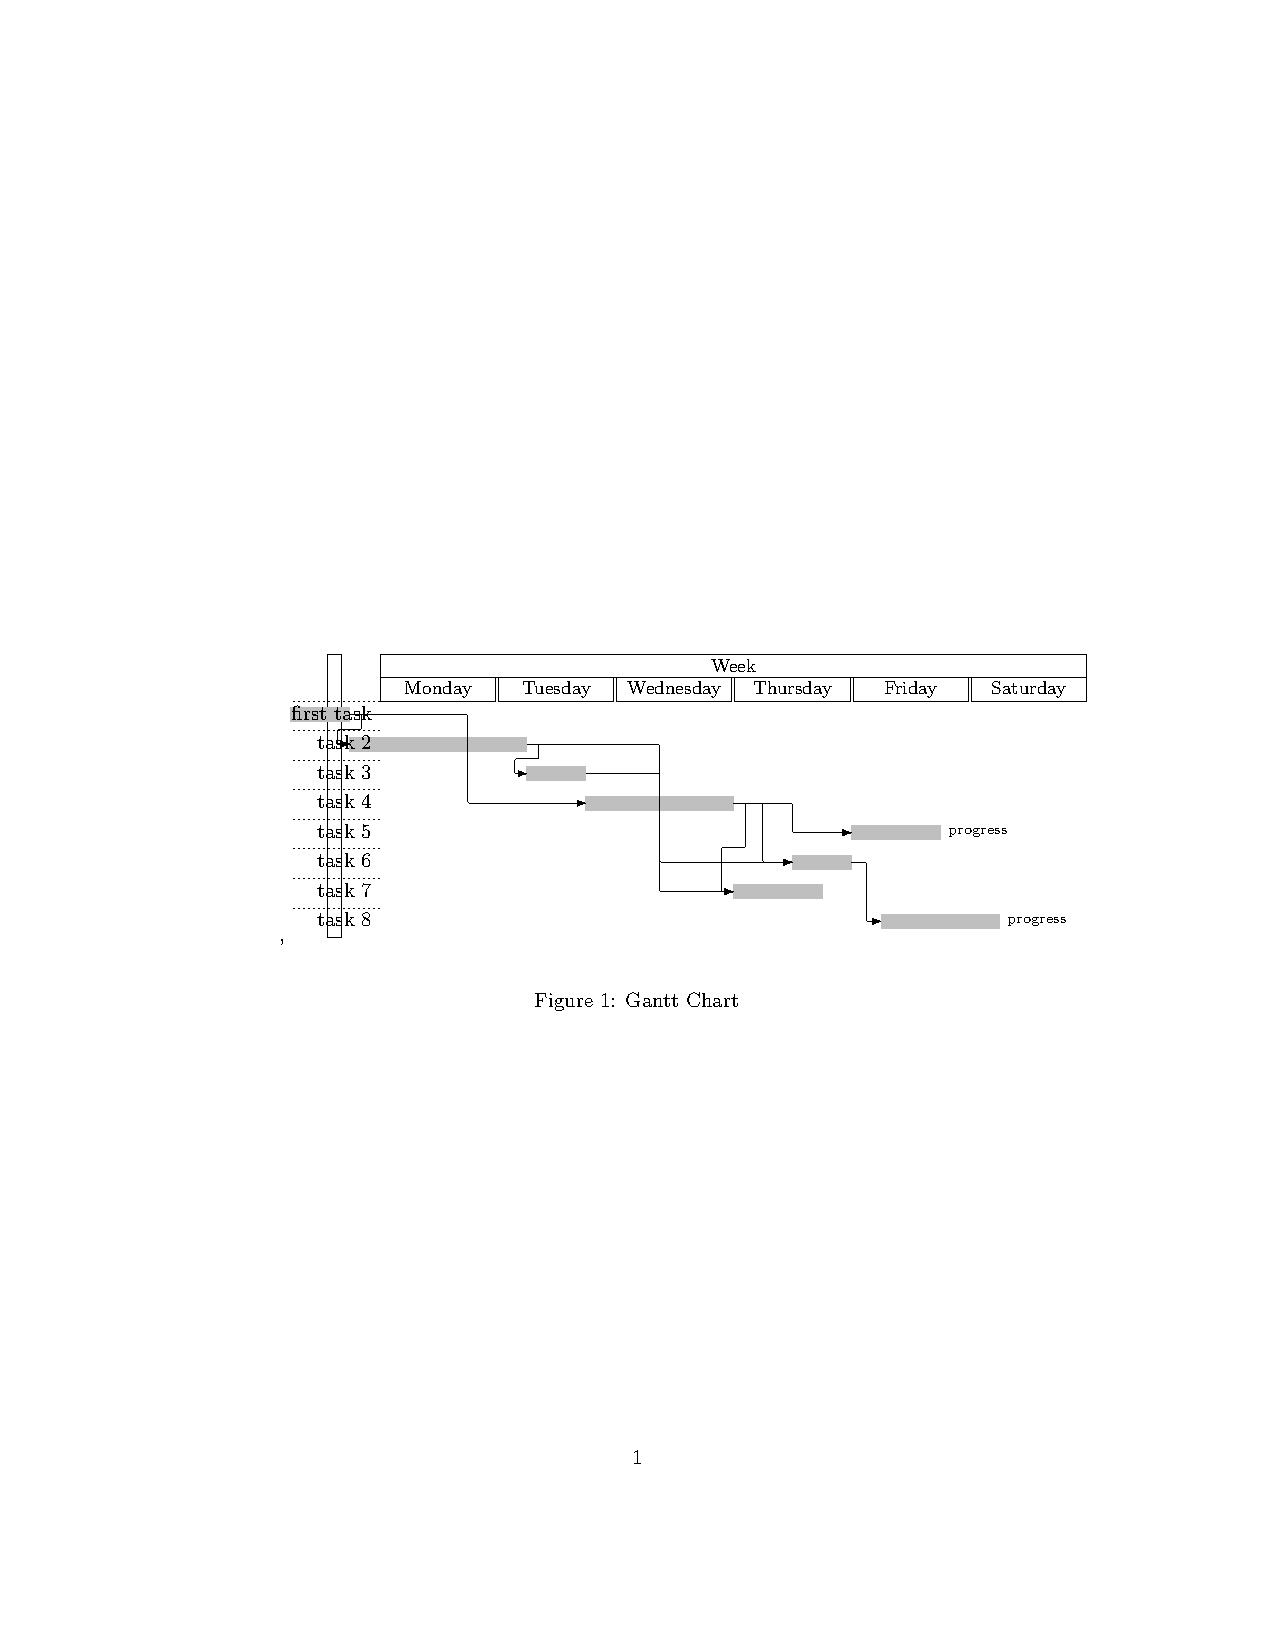
\includegraphics[scale=0.9]{Gantt.png}

%%\begin{figure}[ftbp]
\begin{figure}[h]
%%\begin{figure}
\begin{center}

\definecolor{RoyalBlue}{RGB}{153,204,254}
 
\begin{ganttchart}[y unit title=0.4cm,y unit chart=0.5cm,
vgrid,hgrid,
title label anchor/.style={below=-1.6ex},
title/.append style={draw=none, fill=RoyalBlue!50!black},
%title left shift=.05,
title left shift=0,
%title right shift=-.05,
title right shift=0,
title height=1,
%bar/.style={fill=gray!50},
bar/.style={fill=RoyalBlue},
bar incomplete/.style={fill=RoyalBlue},
progress label text={progressing},
bar height=0.3,
group right shift=.4,
group top shift=.6,
group height=.3,
group/.append style={draw=black, fill=green!50},
milestone/.append style={fill=black, rounded corners=3pt},
bar/.append style={fill=red, rounded corners=3pt}
%group peaks={0}{0}{.2}
%]{0}{2},
%vrule/.style={very thick, blue}
%vrule label font=\bfseries
]{0}{23},

%labels

\gantttitle{Week}{24} \\
\gantttitle{Monday}{4} 
\gantttitle{Tuesday}{4} 
\gantttitle{Wednesday}{4} 
\gantttitle{Thursday}{4} 
\gantttitle{Friday}{4} 
\gantttitle{Saturday}{4} \\

%tasks
\ganttgroup{Group 1}{1}{10} \\
\ganttbar[progress=50]{Inception}{1}{2} \\
\ganttbar{Feasability study}{3}{8} \\
\ganttbar{Clearchoice}{9}{10} \\
\ganttbar{Proof of concept}{11}{15} \\
\ganttbar[progress=33]{Specifications}{20}{22} \\
\ganttbar{Internal design}{18}{19} \\
\ganttbar{External design}{16}{18} \\
\ganttbar[progress=0]{Release}{21}{23}\\
\ganttbar[progress=0]{task 8}{2}{21}\\
\ganttbar[progress=0]{task 8}{2}{21}\\
\ganttbar[progress=0]{task 8}{2}{21}\\
\ganttbar[progress=0]{task 8}{2}{21}\\
\ganttbar[progress=0]{task 8}{2}{21}\\

%\ganttvrule[
%vrule/.append style={red, thin},
%vrule offset=.2
%]{day z}{6}

%milestones
\ganttmilestone{Milestone 1}{11}

%relations

\ganttlink{elem0}{elem1}
\ganttlink{elem0}{elem3}
\ganttlink{elem1}{elem2}
\ganttlink{elem3}{elem4}
\ganttlink{elem1}{elem5}
\ganttlink{elem3}{elem5}
\ganttlink{elem2}{elem6}
\ganttlink{elem3}{elem6}
\ganttlink{elem5}{elem7}
%\ganttlink{elem8}{elem9}

\end{ganttchart}

\end{center}

\caption{Gantt Chart}

\end{figure}


%%
%%\begin{figure}[ftbp]
\begin{figure}[h]
%%\begin{figure}
\begin{center}

\definecolor{RoyalBlue}{RGB}{153,204,254}
 
\begin{ganttchart}[y unit title=0.4cm,y unit chart=0.5cm,
vgrid,hgrid,
title label anchor/.style={below=-1.6ex},
title/.append style={draw=none, fill=RoyalBlue!50!black},
%title left shift=.05,
title left shift=0,
%title right shift=-.05,
title right shift=0,
title height=1,
%bar/.style={fill=gray!50},
bar/.style={fill=RoyalBlue},
bar incomplete/.style={fill=RoyalBlue},
progress label text={progressing},
bar height=0.3,
group right shift=.4,
group top shift=.6,
group height=.3,
group/.append style={draw=black, fill=green!50},
milestone/.append style={fill=black, rounded corners=3pt},
bar/.append style={fill=red, rounded corners=3pt}
%group peaks={0}{0}{.2}
%]{0}{2},
%vrule/.style={very thick, blue}
%vrule label font=\bfseries
]{0}{23},

%labels

\gantttitle{Week}{24} \\
\gantttitle{Monday}{4} 
\gantttitle{Tuesday}{4} 
\gantttitle{Wednesday}{4} 
\gantttitle{Thursday}{4} 
\gantttitle{Friday}{4} 
\gantttitle{Saturday}{4} \\

%tasks
\ganttgroup{Group 1}{1}{10} \\
\ganttbar[progress=50]{Inception}{1}{2} \\
\ganttbar{Feasability study}{3}{8} \\
\ganttbar{Clearchoice}{9}{10} \\
\ganttbar{Proof of concept}{11}{15} \\
\ganttbar[progress=33]{Specifications}{20}{22} \\
\ganttbar{Internal design}{18}{19} \\
\ganttbar{External design}{16}{18} \\
\ganttbar[progress=0]{Release}{21}{23}\\
\ganttbar[progress=0]{task 8}{2}{21}\\
\ganttbar[progress=0]{task 8}{2}{21}\\
\ganttbar[progress=0]{task 8}{2}{21}\\
\ganttbar[progress=0]{task 8}{2}{21}\\
\ganttbar[progress=0]{task 8}{2}{21}\\

%\ganttvrule[
%vrule/.append style={red, thin},
%vrule offset=.2
%]{day z}{6}

%milestones
\ganttmilestone{Milestone 1}{11}

%relations

\ganttlink{elem0}{elem1}
\ganttlink{elem0}{elem3}
\ganttlink{elem1}{elem2}
\ganttlink{elem3}{elem4}
\ganttlink{elem1}{elem5}
\ganttlink{elem3}{elem5}
\ganttlink{elem2}{elem6}
\ganttlink{elem3}{elem6}
\ganttlink{elem5}{elem7}
%\ganttlink{elem8}{elem9}

\end{ganttchart}

\end{center}

\caption{Gantt Chart}

\end{figure}

[htpb]
%%\includeonly{ProjectGantt}
\end{center}
\lstinputlisting[language=Octave, firstline=3, lastline=5]{../Perl/readCharges}
Let's create a new group for each team involved (owning a deliverable)...\\

\subsection{Events}
From events (Meetings, Deliverables)
\begin{longtable}{|c|c|c|c|}
\hline
\multicolumn{4}{|c|}{Events} \\
\hline
Date & Type & Name & Template\\
\hline
0000-00-00 00:00:00 & Deliverable & Inception & Inception.tex\\
\hline
0000-00-00 00:00:00 & Deliverable & Specification & Specification.tex\\
\hline
0000-00-00 00:00:00 & Deliverable & Clearchoice & Clearchoice.tex\\
\hline
0000-00-00 00:00:00 & Deliverable & External design & External design.tex\\
\hline
0000-00-00 00:00:00 & Deliverable & Internal design & Internal design.tex\\
\hline
0000-00-00 00:00:00 & Deliverable & Test documentation & Test documentation.tex\\
\hline
0000-00-00 00:00:00 & Deliverable & Release notes & Release notes.tex\\
\hline
0000-00-00 00:00:00 & Deliverable & Post implementation review & Post implementation revie\\
\hline
0000-00-00 00:00:00 & Deliverable & Support documentation & Support documentation.tex\\
\hline
0000-00-00 00:00:00 & Deliverable & Inception & Inception.tex\\
\hline
0000-00-00 00:00:00 & Deliverable & Specification & Specification.tex\\
\hline
0000-00-00 00:00:00 & Deliverable & Clearchoice & Clearchoice.tex\\
\hline
0000-00-00 00:00:00 & Deliverable & External design & External design.tex\\
\hline
0000-00-00 00:00:00 & Deliverable & Internal design & Internal design.tex\\
\hline
0000-00-00 00:00:00 & Deliverable & Test documentation & Test documentation.tex\\
\hline
0000-00-00 00:00:00 & Deliverable & Release notes & Release notes.tex\\
\hline
0000-00-00 00:00:00 & Deliverable & Post implementation review & Post implementation revie\\
\hline
0000-00-00 00:00:00 & Deliverable & Support documentation & Support documentation.tex\\
\hline
0000-00-00 00:00:00 & Birthday & Annif Antoine & Annif Antoine.tex\\
\hline
0000-00-00 00:00:00 & Meeting & Council & Council.tex\\
\hline
0000-00-00 00:00:00 & Daily & Daily setup & ManagementSummary.pdf\\
\hline
0000-00-00 00:00:00 & Event & Renewal Ins Auto & Letter.pdf\\
\hline
0000-00-00 00:00:00 & Event & Renewal Ins Bateau & Letter.pdf\\
\hline
0000-00-00 00:00:00 & Event & Renewal Ins Maison & Letter.pdf\\
\hline
0000-00-00 00:00:00 & Event & Car servicing & Letter.pdf\\
\hline
0000-00-00 00:00:00 & Event & Renewal paiment card & Letter.pdf\\
\hline
0000-00-00 00:00:00 & Event & Taxes declaration & Letter.pdf\\
\hline
0000-00-00 00:00:00 & Event & Taxes paiement & Letter.pdf\\
\hline
0000-00-00 00:00:00 & Event & Christmas tree Apologic & Letter.pdf\\
\hline
0000-00-00 00:00:00 & Event & Birthday me & Birthday me.tex\\
\hline
0000-00-00 00:00:00 & Event & Birthday Juliette & Birthday Juliette.tex\\
\hline
0000-00-00 00:00:00 & Event & Birthday Thibault & Birthday Thibault.tex\\
\hline
0000-00-00 00:00:00 & Event & Birthday Emilie & Birthday Emilie.tex\\
\hline
0000-00-00 00:00:00 & Event & Birthday Antoine & Birthday Antoine.tex\\
\hline
0000-00-00 00:00:00 & Event & Poker tour St Meen & Poker tour St Meen.tex\\
\hline
0000-00-00 00:00:00 & Event & Clean the deck & Clean the deck.tex\\
\hline
0000-00-00 00:00:00 & Event & Fuck yourself & Clean the deck.tex\\
\hline
2000-01-03 00:00:00 & toto &  & \\
\hline
 ... & ... & ... & ... \\
\hline
\hline
\end{longtable}

\lstinputlisting[language=Octave, firstline=3, lastline=5]{../Perl/readEvents}
There is a problem with date formats\\
We can add a link to both the pdf and the tex document\\
We want to sort them by date and filter on the relevant items\\


\subsection{Tasks}
\subsubsection{Tasks aggregated}
Ajouter time to expiry, Feasible time, Feasible Budget, Feasible Complexity/Risks
RAF, Done, Completion perc, Maturity\\
\begin{longtable}{|c|c|c|}
\hline
\multicolumn{3}{|c|}{Tasks} \\
\hline
Project & ROI & Complexity \\
\hline
MyNew project & 10000000 & 1\\
\hline
Admin & 110546 & 10\\
\hline
Climate camp & 30000 & 4\\
\hline
Boat & 15687 & 273\\
\hline
Friends & 12601 & 29\\
\hline
CaMarchee & 3200 & 53\\
\hline
Work & 1000 & 2\\
\hline
IT & 1000 & 35\\
\hline
Guitar & 145 & 329\\
\hline
Finance & 82 & 9\\
\hline
\end{longtable}

\lstinputlisting[language=Perl, firstline=3, lastline=5]{../Perl/readTasks}
\begin{bchart}[min=0,max=350,step=70,unit=k\texteuro]
\bcbar[label=MyNew project]{100000}\\
\smallskip
\bcbar[label=Admin]{1105}\\
\smallskip
\bcbar[label=Climate camp]{300}\\
\smallskip
\bcbar[label=Boat]{156}\\
\smallskip
\bcbar[label=Friends]{126}\\
\smallskip
\bcbar[label=CaMarchee]{32}\\
\smallskip
\bcbar[label=Work]{10}\\
\smallskip
\bcbar[label=IT]{10}\\
\smallskip
\bcbar[label=Guitar]{1}\\
\smallskip
\bcbar[label=Finance]{0}\\
\smallskip
\end{bchart}

\lstinputlisting[language=Perl, firstline=3, lastline=5]{../Perl/readTasks}

%\subsubsection{Tasks 3D burndown}
\subsubsection{Tasks 3D burndown}
%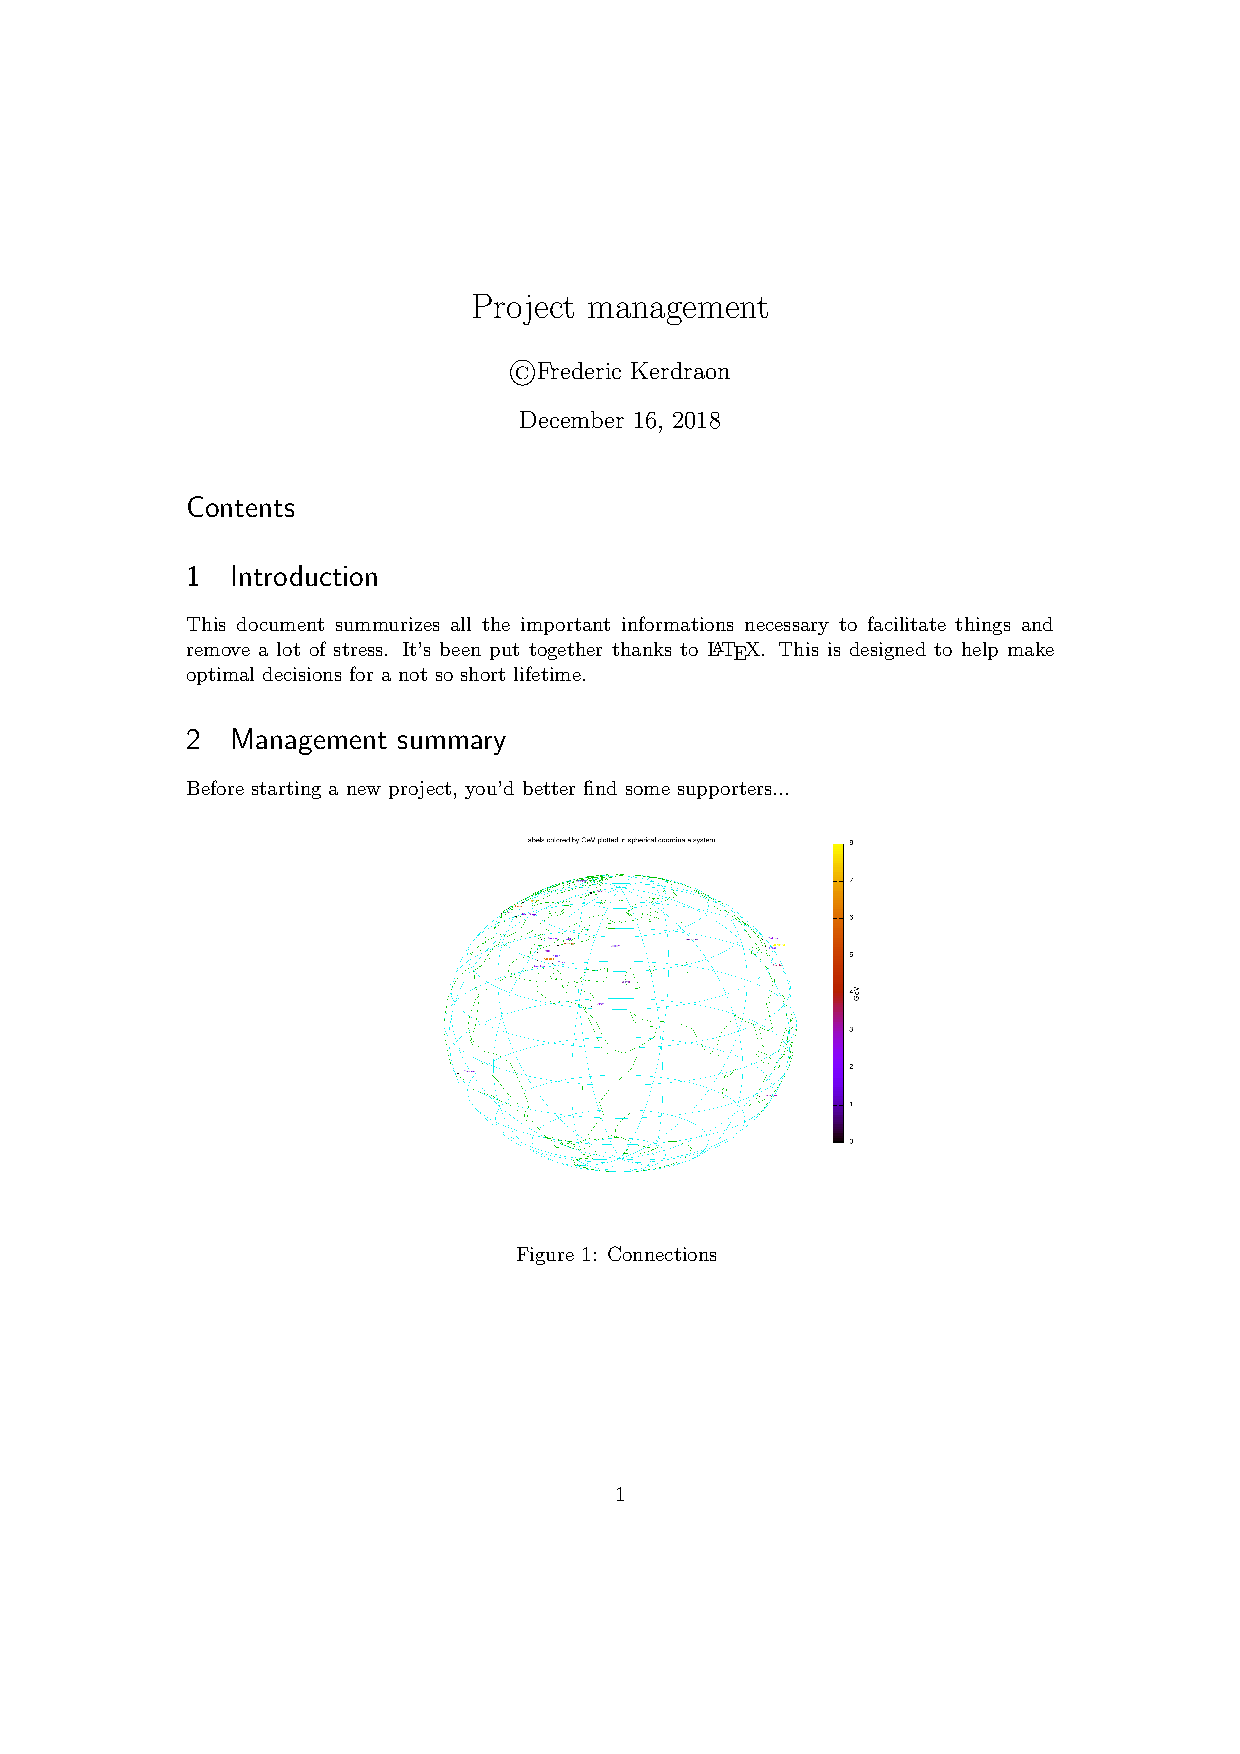
\includegraphics[width=1\textwidth]{Project.png}
\input{Scatter2}
\lstinputlisting[language=Octave, firstline=3, lastline=5]{../Perl/readCharges}
See if we add some text here...\\
%\input{3dTasks}
\includegraphics[scale=0.6]{../Maths/Scilab-burndown.png}
\lstinputlisting[language=Octave, firstline=3, lastline=5]{../Perl/readCharges}
I'm not sure where this is coming from and it looks like a mix of Scilab and Latex...\\
%\includegraphics[width=90mm]{Scilab-burndown.png}

\subsubsection{Tasks detailed}
If the tasks represent a certain amount of the project total, then we should highligt in red.\\
\begin{longtable}{|c|c|c|c|c|c|}
\hline
\multicolumn{6}{|c|}{Tasks} \\
\hline
Project & Task & Return & Cost & R/C & NumDays \\
\hline
MyNew project & toto & 10000000 & 1 & 10000000 & 10\\
\hline
Admin & Vider les poubelles & 100000 & 1 & 100000 & 10\\
\hline
Climate camp & visiter les terrains et poser des jalons & 15000 & 1 & 15000 & 10\\
\hline
Climate camp & visiter les terrains et poser des jalons & 15000 & 1 & 15000 & 10\\
\hline
Boat & Sell Plijadur & 15000 & 1 & 15000 & 10\\
\hline
Admin & Appeler Fanch & 4000 & 1 & 4000 & 10\\
\hline
Admin & Faire le virement Suppletis & 3000 & 1 & 3000 & 10\\
\hline
Admin & Declare revenues & 2000 & 1 & 2000 & 10\\
\hline
Friends & Diner Miss Univers & 1200 & 1 & 1200 & 10\\
\hline
IT & Qt - add global update for tasks from Qt & 1000 & 1 & 1000 & 10\\
\hline
\end{longtable}

\lstinputlisting[language=Octave, firstline=3, lastline=5]{../Perl/readCharges}
\begin{bchart}[min=0,max=50,step=10,unit=k\texteuro]
\bcbar[label=toto]{10000}\\
\smallskip
\bcbar[label=Vider les poubelles]{100}\\
\smallskip
\bcbar[label=visiter les terrains et poser des jalons]{15}\\
\smallskip
\bcbar[label=visiter les terrains et poser des jalons]{15}\\
\smallskip
\bcbar[label=Sell Plijadur]{15}\\
\smallskip
\bcbar[label=Appeler Fanch]{4}\\
\smallskip
\bcbar[label=Faire le virement Suppletis]{3}\\
\smallskip
\bcbar[label=Declare revenues]{2}\\
\smallskip
\bcbar[label=Diner Miss Univers]{1}\\
\smallskip
\bcbar[label=Qt - add global update for tasks from Qt]{1}\\
\smallskip
\end{bchart}

\lstinputlisting[language=Octave, firstline=3, lastline=5]{../Perl/readCharges}


%\subsubsection{ROI}
\subsubsection{Team workload}
%\includegraphics[width=90mm]{Contacts.png}
%\includegraphics[width=90mm]{Projects.png}
%\includegraphics[width=90mm]{EventsPro.png}
%\includegraphics[width=90mm]{Resources.png}
%\includegraphics[width=90mm]{Resources.png}
\input{kiviat5}
%\subsubsection{Budget}
\lstinputlisting[language=Octave, firstline=3, lastline=5]{../Perl/readCharges}
%From Tasks.csv

\subsubsection{Risks}

Not enough budget\\ 
Not enough resources (including me)\\

\subsubsection{Management decisions}

Increase availability from team member 1\\
Allocate new budget for infrastructure\\
External study\\

\subsubsection{Next targets}

Deliver ....\\
Deliver ....\\
Deliver ....\\
Deliver ....\\
%\footnote{Work expands to fill the time available for its completion}

\subsection{Budget}
\includegraphics[scale=0.45]{Charges.png}
\lstinputlisting[language=Octave, firstline=3, lastline=5]{../Perl/readCharges}

\subsubsection{Propositions from Artificial Intelligence}
%\subsubsection{Table}


\section{Associated Project Management}

From now on we focus on one single project, else it's gonna be messie 
\subsection{Deliverables}
From events.csv
\subsection{Gantt}
Pour que le Gantt soit a sa place!!!!!
%\documentclass{article}
%\usepackage{tikz}
%\usetikzlibrary{arrows,shapes,positioning,shadows,trees}

\definecolor{mainblue}{HTML}{6699CC}
%%\definecolor{maingray}{HTML}{B9B9B9}
\definecolor{maingray}{HTML}{91A3B0}

\tikzset{
  basic/.style  = {draw, text width=2cm, drop shadow, font=\sffamily, rectangle},
  root/.style   = {basic, rounded corners=2pt, thin, align=center,
                   fill=mainblue},
  %%level 2/.style = {basic, rounded corners=6pt, thin,align=center, fill=green!60,
  level 2/.style = {basic, rounded corners=6pt, thin,align=center, fill=maingrey,
                   text width=8em},
  level 3/.style = {basic, thin, align=left, fill=pink!60, text width=6.5em}
}

%\begin{document}

\begin{tikzpicture}[
  level 1/.style={sibling distance=40mm},
  edge from parent/.style={->,draw},
  >=latex]

% root of the the initial tree, level 1
\node[root] {Drawing diagrams}
% The first level, as children of the initial tree
  child {node[level 2] (c1) {Defining node and arrow styles}}
  child {node[level 2] (c2) {Positioning the nodes}}
  child {node[level 2] (c3) {Drawing arrows between nodes}};

% The second level, relatively positioned nodes
\begin{scope}[every node/.style={level 3}]
\node [below of = c1, xshift=15pt] (c11) {Setting shape};
\node [below of = c11] (c12) {Choosing color};
\node [below of = c12] (c13) {Adding shading};

\node [below of = c2, xshift=15pt] (c21) {Using a Matrix};
\node [below of = c21] (c22) {Relatively};
\node [below of = c22] (c23) {Absolutely};
\node [below of = c23] (c24) {Using overlays};

\node [below of = c3, xshift=15pt] (c31) {Default arrows};
\node [below of = c31] (c32) {Arrow library};
\node [below of = c32] (c33) {Resizing tips};
\node [below of = c33] (c34) {Shortening};
\node [below of = c34] (c35) {Bending};
\end{scope}

% lines from each level 1 node to every one of its "children"
\foreach \value in {1,2,3}
  \draw[->] (c1.195) |- (c1\value.west);

\foreach \value in {1,...,4}
  \draw[->] (c2.195) |- (c2\value.west);

\foreach \value in {1,...,5}
  \draw[->] (c3.195) |- (c3\value.west);
\end{tikzpicture}


\lstinputlisting[language=Octave, firstline=3, lastline=5]{../Perl/readCharges}
%\input{Gantt2}
%#####################################################################################

\subsection{Global Burn down}
From tasks.csv + Dispo weekly of each resource
%Graphique\\

\input{Regression}
\\
Calcul de vitesse\\
s=speed\\
p=position\\
n=number of units\\
t=time\\
s=n/t\\
\\
Projection lineaire\\
y=s*x+p\\
Theoretical end\\
\lstinputlisting[language=Octave, firstline=3, lastline=5]{../Perl/readCharges}

%\includegraphics[width=20pts]{Geometric.jpg}

\subsubsection{Burndown by team}
%\input{2Din3D}
\input{2Din3D_new}
\\
Calcul de vitesse\\
s=speed\\
p=position\\
n=number of units\\
t=time\\
s=n/t\\
\\
Projection lineaire\\
y=s*x+p\\
Theoretical end\\
\lstinputlisting[language=Octave, firstline=3, lastline=5]{../Perl/readCharges}

%\subsubsection{Yet another Perfect Burndown}
%\input{Scatter2}

\subsection{Resources}

Top 10 resources to take care of\\
Workload (days, percentage time, stress, fatigue sum of days without break, ambition)
Diagramme en etoile per deliverable\\
Rates for all the resources

\subsubsection{Data}
\begin{longtable}{|c|c|c|c|c|}
\hline
\multicolumn{5}{|c|}{Contacts} \\
\hline
ID & Name & Rating & Town & Telephone\\
\hline
125 & Pascalapo & 1000 &  & \\
\hline
128 & Fredport & 950 &  & \\
\hline
126 & Patrickport & 600 &  & \\
\hline
130 & Cathyapo & 500 &  & \\
\hline
129 & Neilport & 300 &  & \\
\hline
132 & C�dricGarApo & 250 &  & \\
\hline
127 & Arnaudport & 200 &  & \\
\hline
133 & Angeport & 180 &  & \\
\hline
131 & C�dricLApo & 100 &  & \\
\hline
134 & Nicoport & 50 &  & \\
\hline
135 & SebTapo & 50 &  & \\
\hline
 ... & ... & ... & ... & ... \\
\hline
Total & 4180 &  & & \\
\hline
\end{longtable}

\lstinputlisting[language=Octave, firstline=3, lastline=5]{../Perl/readResources}
%\subsubsection{Graph}
%\begin{bchart}[min=0,max=1000,step=200,unit=K\texteuro]
\bcbar[label=Pascalapo]{1000}\\
\smallskip
\bcbar[label=Fredport]{950}\\
\smallskip
\bcbar[label=Patrickport]{600}\\
\smallskip
\bcbar[label=Cathyapo]{500}\\
\smallskip
\bcbar[label=Neilport]{300}\\
\smallskip
\bcbar[label=C�dricGarApo]{250}\\
\smallskip
\bcbar[label=Arnaudport]{200}\\
\smallskip
\bcbar[label=Angeport]{180}\\
\smallskip
\bcbar[label=C�dricLApo]{100}\\
\smallskip
\bcbar[label=Nicoport]{50}\\
\smallskip
\bcbar[label=SebTapo]{50}\\
\smallskip
\end{bchart}

\subsubsection{Cheese}
\begin{tikzpicture}[scale=2.5]
\foreach \p/\t in {
23 / Pascalapo-1000K\texteuro ,
22 / Fredport-950K\texteuro ,
14 / Patrickport-600K\texteuro ,
11 / Cathyapo-500K\texteuro ,
7 / Neilport-300K\texteuro ,
5 / C�dricGarApo-250K\texteuro ,
4 / Arnaudport-200K\texteuro ,
4 / Angeport-180K\texteuro ,
2 / C�dricLApo-100K\texteuro ,
1 / Nicoport-50K\texteuro ,
1 / SebTapo-50K\texteuro ,
}
  {
\setcounter{a}{\value{b}}
\addtocounter{b}{\p}
\slice{\thea/100*360}
          {\theb/100*360}
          {\p\%}{\t}
  }
\end{tikzpicture}

\lstinputlisting[language=Octave, firstline=3, lastline=5]{../Perl/readResources}

\subsubsection{Kiviat}
\input{resourcesKiviat}
\lstinputlisting[language=Octave, firstline=3, lastline=5]{../Perl/readResources}

%\subsubsection{Star diagram}
%\setlength{\unitlength}{0.75mm}
%\begin{picture}(80,60)
%\put(30,20){\vector(1,0){30}}
%\put(30,20){\vector(4,1){20}}
%\put(30,20){\vector(3,1){25}}
%\put(30,20){\vector(2,1){30}}
%\put(30,20){\vector(1,2){10}}
%\put(0,3.35){\makebox(0,0){$y$}
%\thicklines
%\put(20,15){\vector(-4,1){35}}
%\put(20,15){\vector(-1,4){10}}
%\thinlines
%\put(30,20){\vector(-1,-1){5}}
%\put(30,20){\vector(-1,-4){5}}
%\end{picture}

\subsection{Tasks}

%{\footnotesize
\begin{longtable}{|c|c|c|c|c|c|}
\hline
\multicolumn{6}{|c|}{Tasks} \\
\hline
Project & Task & Return & Cost & R/C & NumDays \\
\hline
MyNew project & toto & 10000000 & 1 & 10000000 & 10\\
\hline
Admin & Vider les poubelles & 100000 & 1 & 100000 & 10\\
\hline
Climate camp & visiter les terrains et poser des jalons & 15000 & 1 & 15000 & 10\\
\hline
Climate camp & visiter les terrains et poser des jalons & 15000 & 1 & 15000 & 10\\
\hline
Boat & Sell Plijadur & 15000 & 1 & 15000 & 10\\
\hline
Admin & Appeler Fanch & 4000 & 1 & 4000 & 10\\
\hline
Admin & Faire le virement Suppletis & 3000 & 1 & 3000 & 10\\
\hline
Admin & Declare revenues & 2000 & 1 & 2000 & 10\\
\hline
Friends & Diner Miss Univers & 1200 & 1 & 1200 & 10\\
\hline
IT & Qt - add global update for tasks from Qt & 1000 & 1 & 1000 & 10\\
\hline
\end{longtable}

\lstinputlisting[language=Octave, firstline=3, lastline=5]{../Perl/readCharges}
%}

\section{Annexes}

%\subsection{Rate}

%\begin{bchart}[min=0,max=10000,step=5000,unit=\texteuro]
%  \bcbar[label=Daily]{400}
%  \smallskip
%  \bcbar[label=Weekly]{1900}
%  \smallskip
%  \bcbar[label=Monthly]{7600}
%  \smallskip
%  \bcbar[label=3 Months]{10000}
%  \smallskip
  %\medskip
  %\bigskip
%\end{bchart}

\subsection{Tools}

{\footnotesize
\subsubsection{Data}
\input{tools}
\lstinputlisting[language=Octave, firstline=3, lastline=5]{../Perl/readCharges}
%\subsubsection{Graph}
%\input{toolsGraph}
\subsubsection{Cheese}
\input{toolsCheese}
\lstinputlisting[language=Octave, firstline=3, lastline=5]{../Perl/readCharges}
\subsubsection{Architecture}
}

\subsection{Documentations and links}
See References-ok.csv
%\section{Calendars}

%\subsection{Monthly calendar}

%{\footnotesize
%Will contain deliverables, meetings and holidays, republic off\\
%}

%\begin{calendar}{\hsize}
 
%----------------------------------------------------------------------------------------
%	BLANK DAYS BEFORE THE BEGINNING OF THE CALENDAR
%----------------------------------------------------------------------------------------

% This part is very finicky. It defines the number of blank days at the beginning of the calendar before the first of the month starts. If you need this to be more than 4 (i.e. the first starts on a Friday or Saturday in a 31 day month), then you have two options: 
% 1) You can uncomment another one or two \BlankDay's below which will make a new week (6 total) which makes the calendar too big for one page, remedy this by decreasing the size of each day by replacing 2.5cm below with a smaller number. 
% 2) Make the spill-over days start at the top left of the calendar (i.e. the calendar starts with 31 then a few days blank then 1, 2, 3, etc). The second option can be configured by uncommenting the below:

%\setcounter{calendardate}{31} % Begin the count with 31 so the top left day is 31; this can be changed to 29 or 30 as required
%\day{}{\vspace{2.5cm}} % 31 - add another line identical to this if starting at 30 or earlier

% You will need to comment out the 31 in the NUMBERED DAYS AND CALENDAR CONTENT section below for this as well as commenting out one of the \BlankDay's below. Play around with it and you will get it.

%\BlankDay
%\BlankDay
%\BlankDay
%\BlankDay
%\BlankDay
%\BlankDay

%----------------------------------------------------------------------------------------
%	NUMBERED DAYS AND CALENDAR CONTENT
%----------------------------------------------------------------------------------------

% These are the numbered days in the template - if there are less than 31 days simply comment out the bottom lines.

% \vspace{2.5cm} is only there to provide an even look to the calendar where each day is 2.5cm tall, it can be changed or removed to automatically adjust to the day in the week with the most content

%\setcounter{calendardate}{1} % Start the date counter at 1

%\day{Work}{10am Meeting with Boss \\[6pt] 12pm Meeting with Group} % 1 - Example of content
%\day{}{\vspace{2.5cm}} % 2 
%\day{}{\vspace{2.5cm}} % 3
%\day{}{\vspace{2.5cm}} % 4
%\day{}{\vspace{2.5cm}} % 5
%\day{}{\vspace{2.5cm}} % 6
%\day{}{\vspace{2.5cm}} % 7
%\day{}{\vspace{2.5cm}} % 8
%\day{Work}{Start giving classes \\[6pt] Pythagore} % 1 - Example of content
%\day{}{\vspace{2.5cm}} % 9
%\day{Work}{Delivery one \\[6pt] 12pm Meeting with Group} % 1 - Example of content
%\day{}{\vspace{2.5cm}} % 10
%\day{}{\vspace{2.5cm}} % 11
%\day{}{\vspace{2.5cm}} % 12
%\day{Work}{Delivery two \\[6pt] 12pm Meeting with Group} % 1 - Example of content
%\day{}{\vspace{2.5cm}} % 13
%\day{}{\vspace{2.5cm}} % 14
%\day{Perso}{Annif \\[6pt] Cado} % 1 - Example of content
%\day{}{\vspace{2.5cm}} % 15
%\day{}{\vspace{2.5cm}} % 16
%\day{}{\vspace{2.5cm}} % 17
%\day{}{\vspace{2.5cm}} % 18
%\day{}{\vspace{2.5cm}} % 19
%\day{}{\vspace{2.5cm}} % 20 
%\day{}{\vspace{2.5cm}} % 21
%\day{Perso}{Annif \\[6pt] Cado} % 1 - Example of content
%\day{}{\vspace{2.5cm}} % 22
%\day{}{\vspace{2.5cm}} % 23
%\day{}{\vspace{2.5cm}} % 24
%\day{}{\vspace{2.5cm}} % 25
%\day{}{\vspace{2.5cm}} % 26
%\day{}{\vspace{2.5cm}} % 27
%\day{}{\vspace{2.5cm}} % 28
%\day{}{\vspace{2.5cm}} % 29 
%\day{}{\vspace{2.5cm}} % 30 
%\day{}{\vspace{2.5cm}} % 31

% Un-comment the \BlankDay below if the bottom line of the calendar is missing
%\BlankDay

% Un-comment to start counting again after 31
%\setcounter{calendardate}{1}
%\day{}{\vspace{2.5cm}} % 1
%\day{}{\vspace{2.5cm}} % 2
%\day{}{\vspace{2.5cm}} % 3

%----------------------------------------------------------------------------------------

%\finishCalendar
%\end{calendar}

%\subsection{Yearly calendar}

%Mon calendrier annuel\\

\end{document}
